\documentclass[11pt]{article}

\usepackage{scrextend}
\usepackage[a4paper, margin = 1.25in,footskip =0.25in]{geometry}
\usepackage{enumitem}
\usepackage{amsmath}
\usepackage{alltt}
\usepackage{amssymb}
\usepackage{amsthm}
\usepackage{mathtools}
\usepackage{amsmath}
\usepackage{graphicx}

\newcommand{\C}{\mathbb{C}}
\newcommand{\Q}{\mathbb{Q}}
\newcommand{\R}{\mathbb{R}}
\newcommand{\Z}{\mathbb{Z}}

\graphicspath{ {images/} }

\DeclarePairedDelimiter\ceil{\lceil}{\rceil}
\DeclarePairedDelimiter\floor{\lfloor}{\rfloor}

\usepackage{times}

\begin{document}
\begin{flushleft}
	Rowan Lochrin \\
	CSC445 - Alon Efrat\\
	5/1/18 \\
	Homework 6
\end{flushleft}
\begin{enumerate}
	\item The only convex shape is $A\cap B$. This is because for any two
		points in $p_1,p_2 \in A\cap B$, $p_1,p_2\in A$ and $p_1,p_2\in
		B$. Because both $A$ and $B$ are convex there must be a line
		between $p_1$ and $p_2$ in
		both $A$ and $B$ implying that there is a line between $A
		\cap B$.\\
		\begin{figure}[h]
		  \centering
		      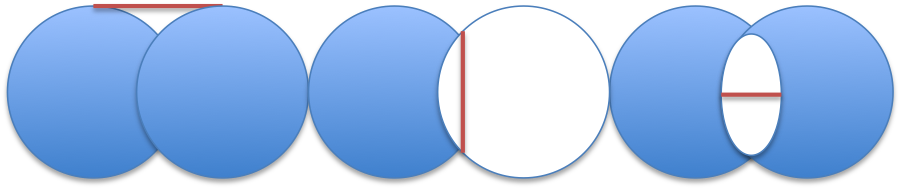
\includegraphics[width=0.65\textwidth]{fig1}
		  \caption{
		Counter examples for $A\cup B$,$A/B$ and $A\Delta B$
		respectively.  }
		\end{figure}
	\item 
		\begin{enumerate}
		\item
			$$y - x \leq 5,
			x \leq 5,
			y \geq 5$$
		\item
			$$y \leq4 ,
			x \leq 5,
			x \leq 6$$
		\item
			$$y - x \leq -5,
			x \leq 0,
			y \geq 0$$
		\end{enumerate}

	\item
		\textbf{Algorithm:}
		Note that finding a paraxial bounding box is the same as finding
		the highest and lowest $x$ and $y$ coordinates of point in the viability
		region. Naturally these will be at vertices of the bounding
		region. We can find the point with the lowest $x$ coordinate on the
		viability region by applying the $O(n^2)$ incremental algorithm
		discussed in class. \\
		To return the highest $x$ coordinate on the viability region we
		need to make one modification to the \textbf{1DLP} function,
		return the highest source pointed down instead  of the lowest
		source pointed up (we still
		need to make sure that the highest source is above the lowest
		source). The modification we need to make to return the points with
		the highest and $y$ coordinates is to simply replace the terms
		highest and lowest with rightmost and leftmost, and the terms
		upward and downward with left and right. Note that  this means for both
		these points we'll make sure that the leftmost source oriented
		right is to the left of the rightmost source oriented left.\\
		Once we have these four points we can simply draw horizontal
		lines through the highest and lowest $y$ coordinates and
		vertical lines through the highest and lowest $x$ coordinates
		to get our bounding box.\\
		\textbf{Correctness:}
		Largely follows from correctness of incremental algorithm. We
		can see that our modification only modifies the point returns
		and does not interfere with the underlining consideration of the
		viability region (even though we don't find the whole viability
		region we calculate one point from it at a time.)
		\textbf{Runtime:}
		The runtime here is $4$ ties the runtime of the incremental
		algorithm so $O(n^2)$ worst case however if we apply the
		randomized approach mentioned in class we can bring the
		\textit{expected} runtime down to $O(n)$.
	\item .
		\begin{figure}[h]
		  \centering
		      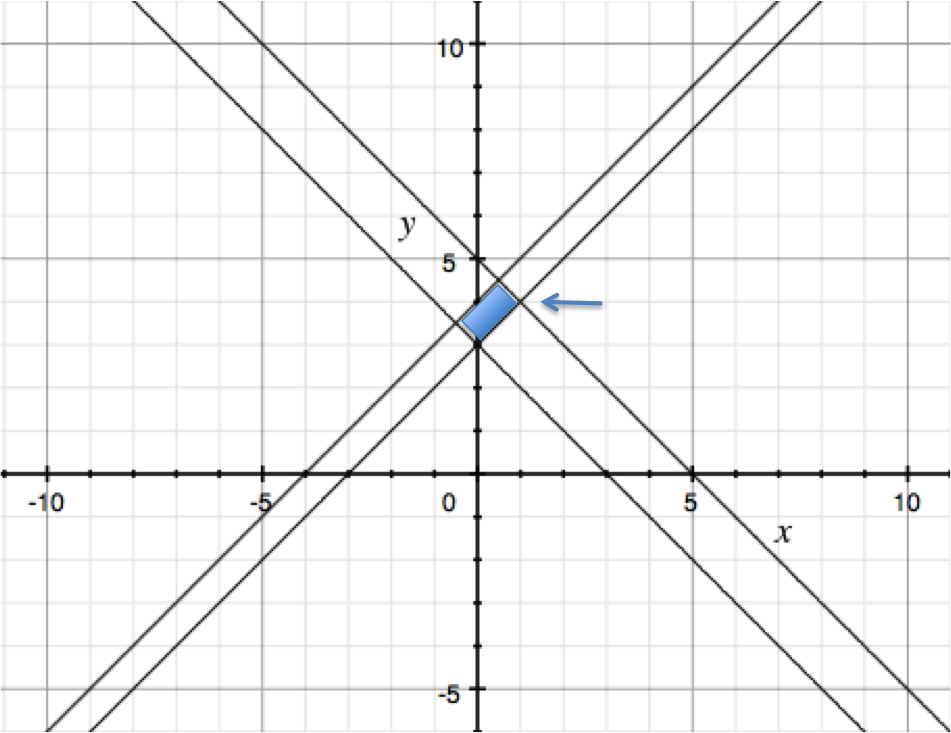
\includegraphics[width=0.65\textwidth]{fig2}
		  \caption{
		We plug in all 4 vertices of the shape to figure out which one
		maximizes the cost function, to find
			$(1,4)$ is our maximum.
		}
		\end{figure}
	\item 

		Define the max and min of $S$ to be the points with the highest
		and lowest $x$-coordinates, respectively.\\
		\textbf{Algorithm:}
		$$ 2\epsilon \leq \max(S) - \min(S) $$
		\textbf{Correctness:}

		Let $q$ be the point in the $x$ axis half way between $\min(S)$
		and $\max(S)$.  If $ 2\epsilon \leq \max(S) - \min(S) $ then
		$|\max(S) - q| = |\min(S) - q| \leq \epsilon $. Because all points
		in $S$ are in between $\min(S)$ and $\max(S)$, we know all points
		are less then $\epsilon$ away from $q$.\\
		We can see that if $ 2\epsilon >  \max(S) - \min(S) $, no point
		$q$ will be $\epsilon$ close to both $\max(S)$ and $\min(s)$.\\
		\textbf{Runtime:}
		$\min$ and $\max$ both run on the order of $O(n)$ so our
		algorithm does as well.
		\textbf{Linear Programming:}
		We could also phrase this as a linear programming problem in one
		dimension with the following equations, where $p_1,...,p_n$ are
		the $x$ values of points in our set.
		$$ p_1 - \epsilon < q <  p_1 + \epsilon$$
		$$ p_2 - \epsilon < q <  p_2 + \epsilon$$
		$$...$$
		$$ p_n - \epsilon < q <  p_n + \epsilon$$
		However we can see that if $p_m$ is the $x$ value of the minimum
		point and $p_M$ is that of maximum point then
		$ p_m + \epsilon > q$, and $p_m - \epsilon < q$
		contain all the information contained in
		the equations above. That is to say all other equations
		represent looser bounds so we need not consider them.
	\item 
		For any point $p$ let $p[x]$, and $p[y]$ be that point's $x$ and
		$y$-coordinates, respectively. We can see that if a point $p_i$
		is above the line, that $\alpha p[x] + \beta \leq p[y]$, so the
		linear programming problem we wish to solve is to find $\alpha $
		and $\beta$ such that 
		\begin{align*}
			\alpha p_1[x] + \beta & \leq p_1[y] &
			\alpha q_1[x] + \beta & \geq q_1[y] \\
			\alpha p_2[x] + \beta & \leq p_2[y] &
			\alpha q_2[x] + \beta & \geq q_2[y] \\
			.... & & ...\\
			\alpha p_n[x] + \beta & \leq p_n[y] &
			\alpha q_n[x] + \beta & \geq q_n[y] \\
		\end{align*}
		
		From here, we can use an unmodified simplex algorithm discussed
		in class to solve this for $\alpha$ and $\beta$, so in the worst case the runtime of this
		algorithm is non-polynomial, but in practice simplex usually
		finishes much faster.
		For $\alpha$ and $\beta$ with an expected time on the order of
		$O(n)$ (worse case $O(n^2)$) where $n$ is the number of points we wish to
		separate. 
	\item The approach here is mostly the same as in the last question.
		However for this problem, we don't want to draw a line
		that divides the points. We seek to draw one that's epsilon close
		to every line. So
		$$ |\alpha p[x] + \beta - p[y] | < \epsilon $$
		which yields the two linear equations
		$ \alpha p[x] + \beta > p[y] - \epsilon $ and 
		$ \alpha p[x] + \beta < p[y] + \epsilon $,
		meaning that for every point $p_i$,
		\begin{align*}
			\alpha p_1[x] + \beta & < p_1[y] + \epsilon &
			\alpha p_1[x] + \beta & > p_1[y] - \epsilon \\
			\alpha p_2[x] + \beta & < p_2[y] + \epsilon &
			\alpha p_2[x] + \beta & > p_2[y] - \epsilon \\
			.... & & ...\\
			\alpha p_n[x] + \beta & < p_n[y] + \epsilon &
			\alpha p_n[x] + \beta & > p_n[y] - \epsilon \\
		\end{align*}
		
\end{enumerate}
\end{document}
